\section{Theorie}
\label{sec:Theorie}

\subsection{Polarisation, Interferenz und Kohärenz}
\label{sec:polarisation}
\subsection{Interferenz und Kohärenz von Licht}
Licht wird in diesem Versuch als stehende elektromagnetische Welle betrachtet, um Interferenzerscheinungen erklären zu können. Die elektrische Feldstärke ist 
ebenfalls eine solche Welle und kann über 
\begin{equation*}
    \vec{E} = \vec{E}_0\cos{(kx- \omega t+ \delta)}
\end{equation*}
beschrieben werden. Die Ausbreitung von Licht wird dabei über die Maxwellschen Gleichungen beschrieben. Außerdem folgt das elektrische Feld 
$\vec{E}$ dem Prinzip der linearen Superposition.
Die Intensität berechnet sich durch 
\begin{equation*}
    I = \langle E^2\rangle _{\text{T}} \; ,
\end{equation*}
wobei $\langle E^2\rangle _{\text{T}}$ nichts anderes als der zeitliche Mittelwert in einem Intervall T ist
\begin{equation*}
    \langle f(t) \rangle _{\text{T}} = \frac{1}{T}\int_t^{t+T} f(t')\text{d}t \, .
\end{equation*}
Da $E$ aus einer überlagerung von zwei Wellen besteht, wird $E=(E_1+E_2)$ gesetzt, wodurch $E^2= E_1^2+E_2^2+2E_1\, E_2$ folgt.
Bei einer Überlagerung von zwei Wellen ergibt sich für die Intensität 
\begin{equation*}
    I = I_1 +I_2 +I_{12}\; .
\end{equation*}
Der Ausdruck $I_{12}$ beschreibt hierbei den Interferenzterm.
Nimmt man an, dass $I_1=I_2$ gilt, so folgt, dass
wenn die Bedingung
\begin{equation*}
    \delta_2 -\delta_1 = \left(2n+1\right)\pi 
\end{equation*}
erfüllt ist, sich die Intensität zu null ergibt und
bei 
\begin{equation*}
    \delta_2 -\delta_1 = \left(2n\right)\pi 
\end{equation*}
sich ein Intesitätsmaximum der Stärke $I=4I_1cos^2{\left(\frac{\delta}{2}\right)}$ zeigt.

Bei zwei unabhängigen Lichtquellen, sind die Phasenkonstanten $\delta_1$ und $\delta_2$ statistische Funktionen der Zeit, wodurch es keine 
Interferenzerscheinung gibt. Dieses Licht ist dann inkohärent. Mithilfe eines LASERs (light amplification by stimulated emission of radiation)
ist es jedoch möglich kohärentes Licht zu erzeugen, welches ein festes $k$, $\omega$ und $\delta$ besitzt.
Bei einem Wegunterschied der einzelnen Strecken des Interferometers, der der Kohärenzlänge $l$ oder mehr entspricht, verschwindet jedoch die 
Interferenzerscheinung. Die Kohärenzlänge berechnet sich über
\begin{equation*}
    l = \text{N}\lambda \; .
\end{equation*}
Dabei ist N die Anzahl der bei beobachtbaren Intensitätsmaxima. $\tau$ ist die Kohärenzzeit. 

%\begin{figure}
%    \centering
    %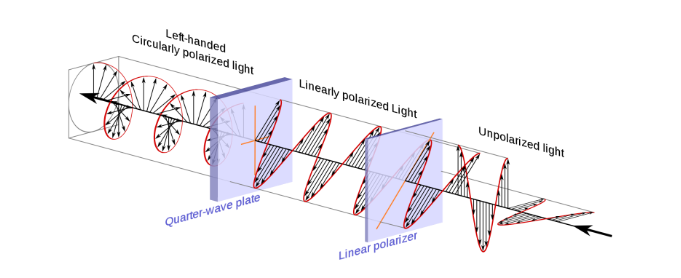
\includegraphics[width = 0.7 \linewidth]{pictures/polarisation1.pdf}
%    \caption{Eine linear polarisierte Welle \cite{demtroeder2}.}
%    \label{fig:polarisation1}
%\end{figure}


\subsection{Kontrast} \label{sec:kontrast}
Als Kontrast (oder Sichtbarkeit) eines Interferometers wird die Beziehung
\begin{equation} \label{eqn:kontrast}
    V = \frac{I_\text{max} - I_\text{min}}{I_\text{max} + I_\text{min}}
\end{equation}
bezeichnet. Offensichtlich gilt also für den Kontrast: $V \in [0,1]$.
Hierbei beschreibt $V$ die Qualität und Deutlichkeit des Interferenzbildes. Hat $V$ den Wert 1, so ist das Minimum nicht sichtbar. Je stärker das Minimum sichtbar ist, desto kleiner wird $V$ bis es den Wert 0 erreicht und keine Interferenz mehr zu erkennen ist.

Für die Intensitätsmaxima/- und minima gilt die Beziehung
\begin{equation*}
    I_\text{max/min} \propto I_\text{Laser} \left[ 1 \pm 2 \cos(\Phi) \sin (\Phi) \right] \, ,
\end{equation*}
aus der sich wiederrum mit \autoref{eqn:kontrast} die Gleichung
\begin{align}\label{eqn:kontrast2}
    V = V(\Phi) &\propto \left|\frac{\left[ 1 + 2 \cos(\Phi) \sin (\Phi) \right] - \left[ 1 - 2 \cos(\Phi) \sin (\Phi) \right]}{\left[ 1 + 2 \cos(\Phi) \sin (\Phi) \right] + \left[ 1 - 2 \cos(\Phi) \sin (\Phi) \right]}\right| \\
    &= \left|2 \cos(\Phi) \sin(\Phi) \right| = \left| \sin (2 \Phi) \right|
\end{align}
ergibt. %Hieraus ist auch sofort ersichtlich, dass der Kontrast bei ungefähr $45°$ am höchsten sein dürfte, wenn alle anderen Einflüsse optimiert sind.

\subsection{Brechungsindex} \label{sec:n}

Der Brechungsindex ist eine intrinsische Eigenschaft eines Materials und kann mittels Interferometer bestimmt werden. Ein Medium mit einem Brechungsindex $n_\text{Medium} > 1$ reduziert die Geschwindigkeit des einfallenden Lichts, was durch die Gleichung
\begin{equation*}
    v_\text{Medium} = \frac{c}{n}
\end{equation*}
beschrieben wird. Ein Lichtstrahl, der durch ein Medium geleitet wird, erfährt eine Phasenverschiebung. Diese Phasenverschiebung kann in Interferometern genutzt werden, um den Brechungsindex eines Mediums zu bestimmen.

Für die Phasenverschiebung in Luft gilt
\begin{equation} \label{eq:nluft}
    \Delta \Phi = \frac{2 \pi}{\lambda_\text{vac}} \Delta n \cdot L \, ,
\end{equation}
wobei $L$ die Länge der evakuierten Zelle ist. Durch Einsetzen der Beziehung der gezählten Intensitätsmaxima 
\begin{equation} \label{eq:maxima}
    M = \frac{\Delta \phi}{2 \pi}
\end{equation}
in \autoref{eq:nluft} lässt sich der Brechungsindex bestimmen:
\begin{align} \label{eq:nluft2}
    \Delta n &= n_\text{Luft} - n_\text{Vak} = \frac{M \cdot \lambda_\text{vac}}{L} \nonumber \\
    n_\text{Luft} &= \frac{M \cdot \lambda_\text{vac}}{L} + 1
\end{align}

Mithilfe des Lorentz-Lorenz-Gesetzes lässt sich der Brechungsindex unter Normalbedingungen berechnen. Das Lorentz-Lorenz-Gesetz lautet
\begin{equation*}
    \frac{n^2 - 1}{n^2 + 2} = \frac{A p}{R T} \, ,
\end{equation*}
wobei $A$ die Refraktivität beschreibt und $R$ die allgemeine Gaskonstante. Nach einer Taylorentwicklung ergibt sich
\begin{equation*}
    n(p) \approx \frac{2 (n-1)}{3} \, ,
\end{equation*} 
woraus sich dann
\begin{equation} \label{eq:lorentz}
    n (T,p) \approx \frac{3 A p}{ 2 R T} + 1
\end{equation}
ergibt.

In diesem Experiment wird auch der Brechungsindex von Glas bestimmt. Für den Brechungsindex in Glas gilt
\begin{equation}\label{eq:phiglas}
    \Delta \phi = \frac{2\pi}{\lambda}T\left(\frac{n-1}{2n}\Delta \theta^2+O( \Delta \theta^4)\right) \, .
\end{equation}
Diese Gleichung wird modifiziert, da zwei Glasplättchen verbaut sind und um $\Theta_0 = \pm 10°$ verkippt sind. Damit ergibt sich die Gleichung in führender Ordnung
\begin{equation}
    \Delta \phi = \frac{\pi \cdot (n - 1) T}{\lambda \cdot n} \left(\left( \theta + 10° \right)^2 - \left( \theta - 10° \right)^2\right) \, ,
\end{equation}
was mit \autoref{eq:maxima} auf die Gleichung
\begin{equation*}
    M = \frac{n - 1}{\lambda \cdot n} \cdot 2 \theta \cdot |\theta_0|
\end{equation*}
und somit auf
\begin{equation} \label{eq:n_Glas}
    n = \frac{1}{1- \frac{\lambda M}{ 2 \theta \cdot |\theta_0| T}}
\end{equation}
führt.